\begin{frame}[fragile]{Intro: Robot Environment} % some commands, e.g. \verb require [fragile]
\begin{center}
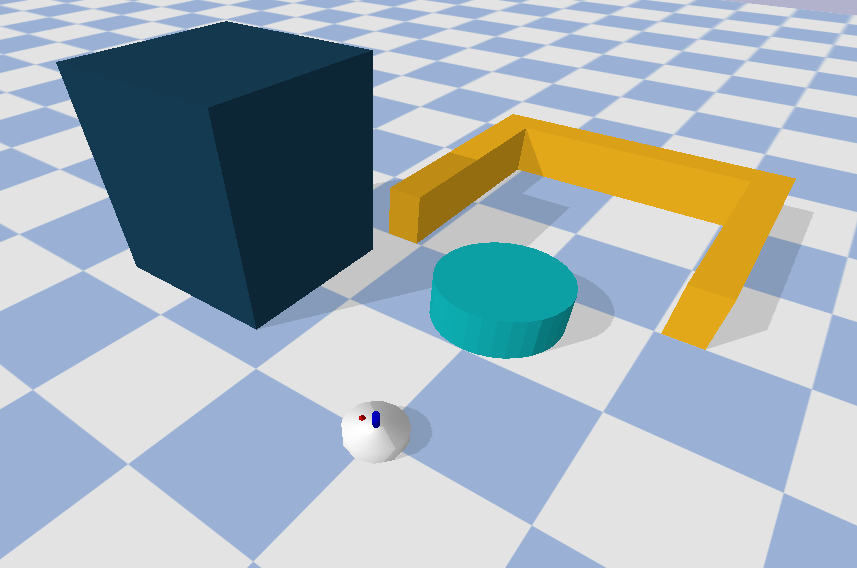
\includegraphics[width=1.0\textwidth]{figures/introduction/blockade}
\end{center}
\end{frame}

\begin{frame}[fragile]{Intro: Thesis Goal} % some commands, e.g. \verb require [fragile]
\begin{itemize}
  \item Learning System Models\\%\pause, <-- put these in here later
  \item Navigation Among Movable Objects (NAMO)\\
  \item Nonprehensile Pushing
\end{itemize}
\end{frame}

\begin{frame}[c]{Intro: Overview Proposed Method} % some commands, e.g. \verb require [fragile]
  \vspace{0.3cm}
\centering
\begin{tikzpicture}[scale=1.05, every node/.style={scale=1.05}, node distance = 2cm, auto]
   
  \node [outer sep=0cm] (environment) at (0,0)  {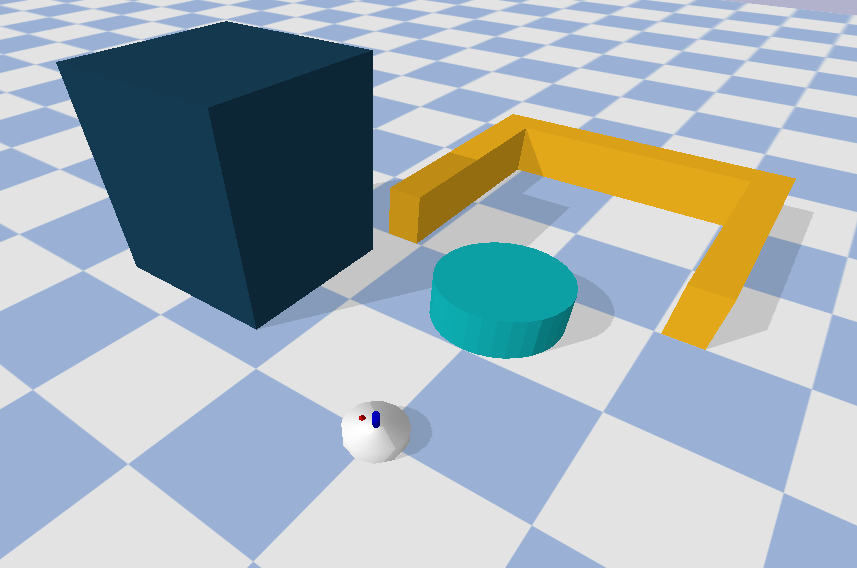
\includegraphics[width=4.6cm]{figures/introduction/blockade}}; overvew

  \draw [myEvenLighterColor,
  rounded corners=0.3cm, 
  line width=0.3cm]  
  (environment.north west) -- 
  (environment.north east) --
  (environment.south east) --
  (environment.south west) -- cycle  ;

  \node [block,
  above of=environment,
  minimum height=2cm,
  minimum width=5cm,
  node distance=4.1cm,
  outer sep=0cm] (hgraph) {Proposed Robot Framework};

  % Draw edges
  \draw[-stealth] ([yshift=0.155cm, xshift=0.4 cm]environment.north) -- node [xshift=-.05cm, right] {\shortstack[]{sensor\\measurements}}([xshift=0.4 cm]hgraph.south) ;
  \draw[-stealth] ([xshift=-0.4 cm]hgraph.south) -- node [left] {robot input}([yshift=0.155cm, xshift=-0.4 cm]environment.north) ;
  \draw[stealth-] (hgraph.west) -- node [above] {task} ++(-1, 0);

\end{tikzpicture}

\end{frame}

\begin{frame}[fragile]{Intro: Research Question}
\large
How do learned objects' system models improve global task planning for a robot with nonprehensile push manipulation abilities over time? \bs

\textbf{Research Subquestions:}
\begin{enumerate}
    \item\label{researchsubquestion:does_it_work}\small How to combine learning and planning for push and drive applications?
    \item\label{researchsubquestion:does_it_compare}\small How does the proposed framework compare against the state-of-the-art?
\end{enumerate}
\end{frame}

\begin{frame}[fragile]{Intro: Task Specification}
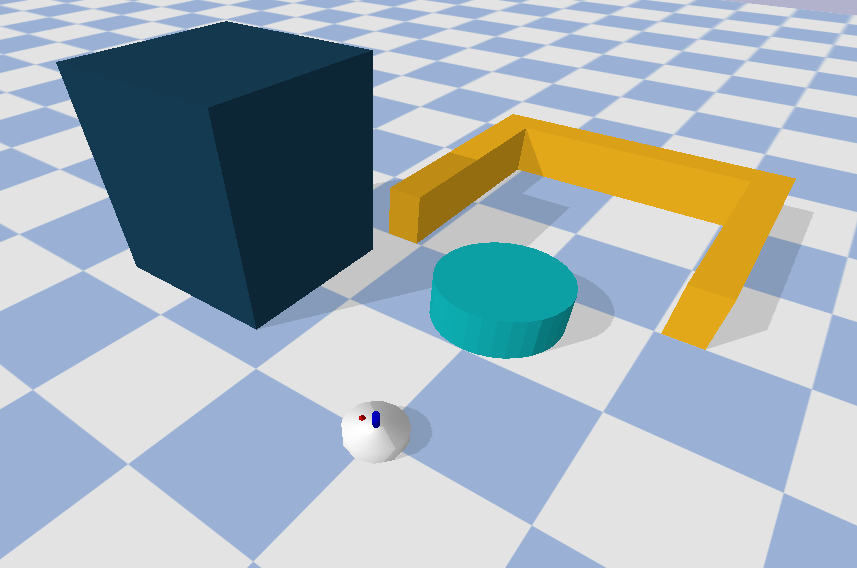
\includegraphics[width=1.0\textwidth]{figures/introduction/blockade}
\end{frame}

\begin{frame}[fragile]{Intro: Task Specification}
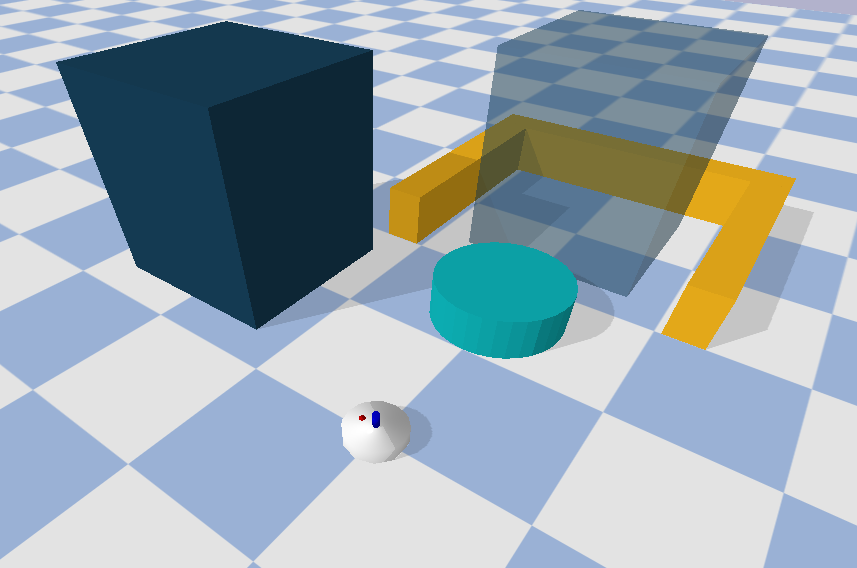
\includegraphics[width=1.0\textwidth]{figures/introduction/blockade_with_target}
\end{frame}

\begin{frame}[fragile]{Assumptions}
\begin{block}{}
\begin{enumerate}
  \item \textbf{Closed-World Assumption:} Objects are manipulated, directly or indirectly only by the robot. Objects cannot be manipulated by influences from outside the environment.\\
\item\textbf{Perfect Object Sensor Assumption:} the robot has full access to the poses and geometry of all objects in the environment at all times.\\
\item\textbf{Tasks are Commutative Assumption:} Tasks consist of multiple objects with specified target positions. The order in which objects are pushed toward their target position is commutative.\\
\item\textbf{Objects do not tip over Assumption:} Movable objects slide if pushed.\\
\end{enumerate}
\end{block}
\end{frame}


\begin{frame}[fragile]{State-of-The-Art}
  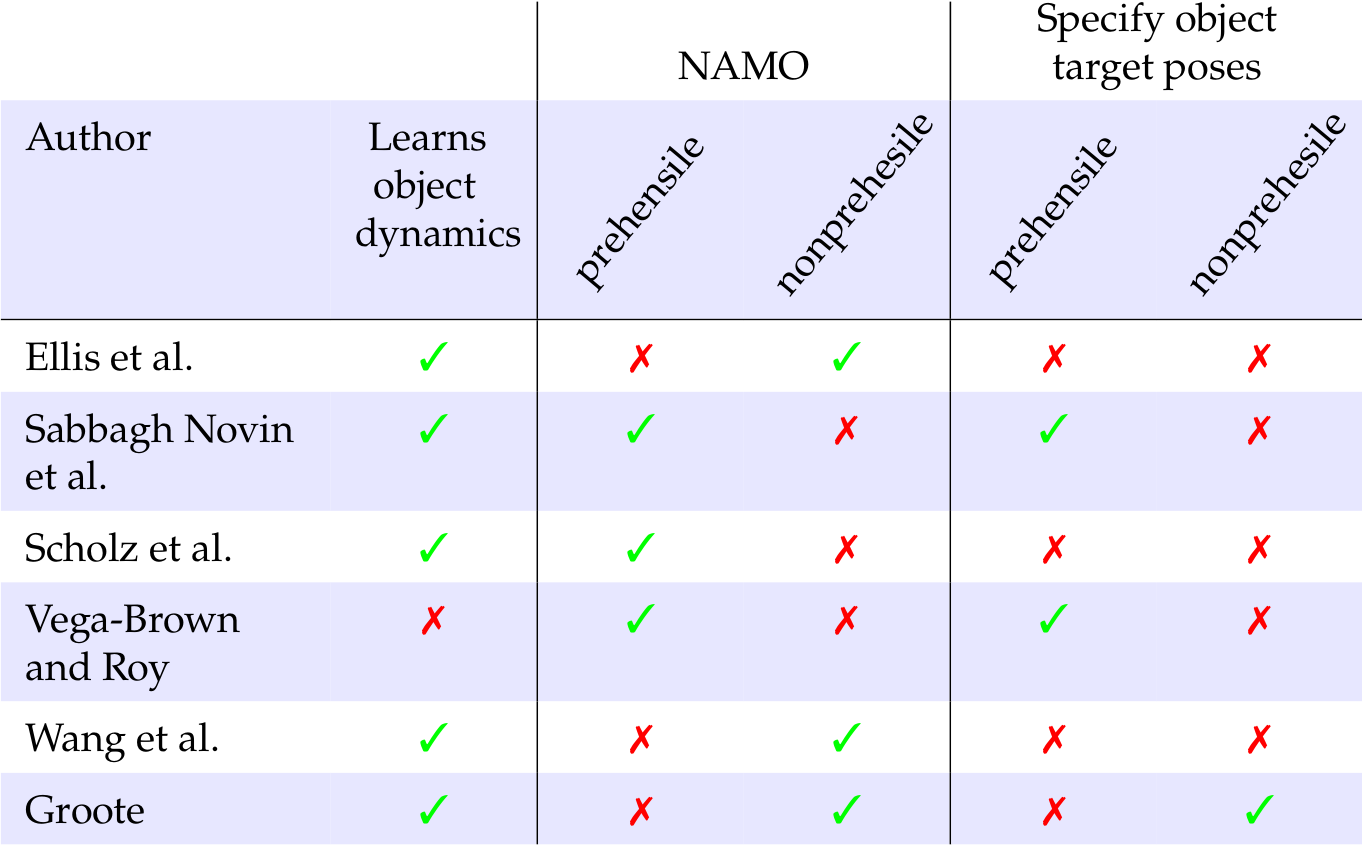
\includegraphics[width=1.0\textwidth]{figures/introduction/sota}

\end{frame}



